\documentclass[tikz, border=8pt]{standalone}
\usepackage{amsmath}
\usepackage{tikz}
\usepackage{ragged2e}
\usetikzlibrary{arrows.meta, calc}

% Compton wavelength macro (matches main.tex definition)
\newcommand{\lambdaC}{\lambda_{\text{C}}}

\begin{document}
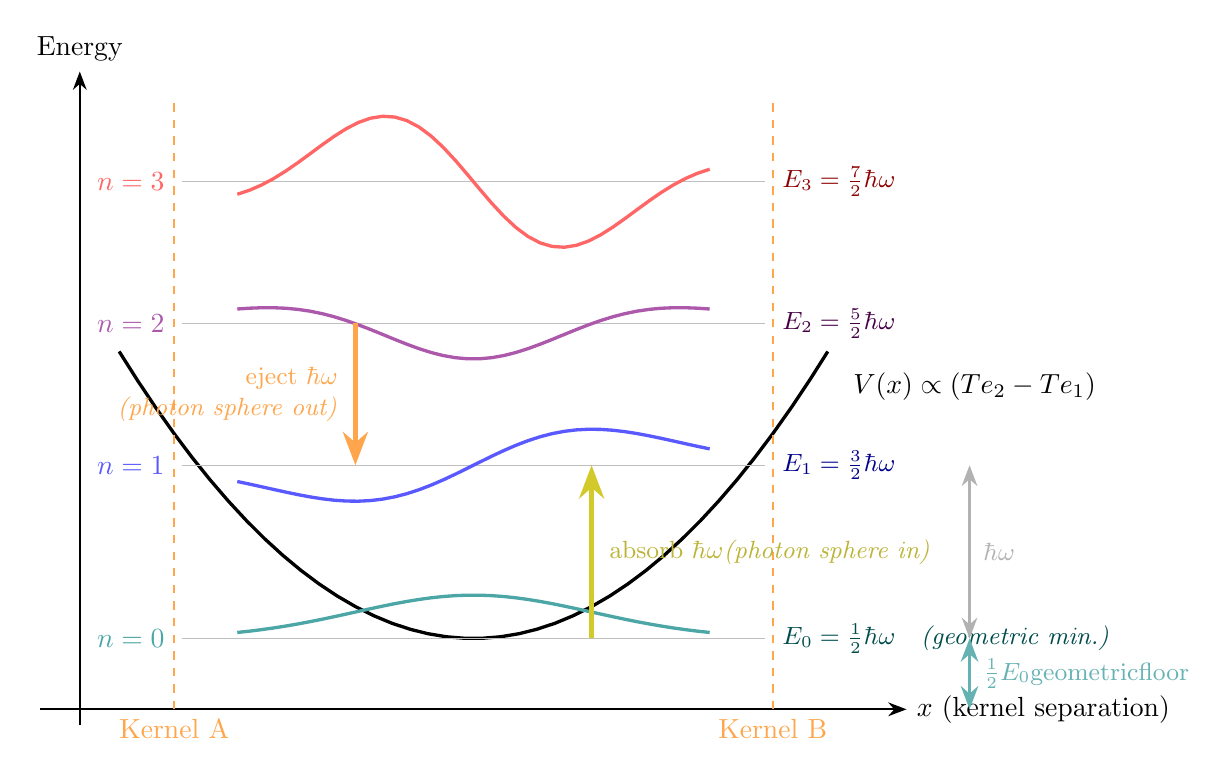
\begin{tikzpicture}[>=Stealth, font=\normalsize]

%% ── Graph elements shifted 1cm to the left ──────────────────
\begin{scope}[xshift=-1cm]

%% ── Axes ─────────────────────────────────────────────────────
\draw[thick, ->] (-5.5, -0.3) -- (5.5, -0.3)
  node[right] {$x$ (kernel separation)};
\draw[thick, ->] (-5.0, -0.5) -- (-5.0, 7.8)
  node[above] {Energy};

%% ── Potential curve (parabola) ───────────────────────────────
\draw[very thick, black]
  plot[domain=-4.5:4.5, samples=40] (\x, {0.18*\x*\x + 0.6});
\node[right, font=\normalsize] at (4.7, 3.8) {$V(x) \propto (Te_2 - Te_1)$};

%% ── Kernel positions ─────────────────────────────────────────
\draw[orange!70, dashed, thick] (-3.8, -0.3) -- (-3.8, 7.5);
\draw[orange!70, dashed, thick] ( 3.8, -0.3) -- ( 3.8, 7.5);
\node[orange!70, below, font=\normalsize] at (-3.8, -0.3) {Kernel A};
\node[orange!70, below, font=\normalsize] at ( 3.8, -0.3) {Kernel B};

%% ── Wavefunctions ────────────────────────────────────────────
%% n=0  (y = 0.6)
\draw[gray!50] (-3.7, 0.6) -- (3.7, 0.6);
\draw[teal!70, very thick]
  plot[domain=-3.0:3.0, samples=40]
  (\x, {0.6 + 0.55*exp(-0.22*\x*\x)});
\node[left, teal!70] at (-3.8, 0.6) {$n=0$};
\node[right, font=\small, teal!60!black] at (3.8, 0.6)
  {$E_0 = \tfrac{1}{2}\hbar\omega$\quad\textit{(geometric min.)}};

%% n=1  (y = 2.8)
\draw[gray!50] (-3.7, 2.8) -- (3.7, 2.8);
\draw[blue!65, very thick]
  plot[domain=-3.0:3.0, samples=40]
  (\x, {2.8 + 0.50*\x*exp(-0.22*\x*\x)});
\node[left, blue!65] at (-3.8, 2.8) {$n=1$};
\node[right, font=\small, blue!55!black] at (3.8, 2.8)
  {$E_1 = \tfrac{3}{2}\hbar\omega$};

%% n=2  (y = 4.6)
\draw[gray!50] (-3.7, 4.6) -- (3.7, 4.6);
\draw[violet!65, very thick]
  plot[domain=-3.0:3.0, samples=40]
  (\x, {4.6 + 0.45*(2*0.22*\x*\x - 1)*exp(-0.22*\x*\x)});
\node[left, violet!65] at (-3.8, 4.6) {$n=2$};
\node[right, font=\small, violet!55!black] at (3.8, 4.6)
  {$E_2 = \tfrac{5}{2}\hbar\omega$};

%% n=3  (y = 6.4)
\draw[gray!50] (-3.7, 6.4) -- (3.7, 6.4);
\draw[red!60, very thick]
  plot[domain=-3.0:3.0, samples=40]
  (\x, {6.4 + 0.40*\x*(2*0.22*\x*\x - 3)*exp(-0.22*\x*\x)});
\node[left, red!60] at (-3.8, 6.4) {$n=3$};
\node[right, font=\small, red!55!black] at (3.8, 6.4)
  {$E_3 = \tfrac{7}{2}\hbar\omega$};

%% ── Transition arrows ────────────────────────────────────────

%% Absorption arrow (n=0 -> n=1): yellow
\draw[->, yellow!80!black, very thick, line width=2.0pt]
  (1.5, 0.6) -- (1.5, 2.8);
\node[right, yellow!70!black, font=\small] at (1.6, 1.7)
  {absorb $\hbar\omega$\\\textit{(photon sphere in)}};

%% Emission arrow (n=2 -> n=1): orange
\draw[->, orange!70, very thick, line width=2.0pt]
  (-1.5, 4.6) -- (-1.5, 2.8);
\node[left, orange!70, font=\small, align=right] at (-1.6, 3.7)
  {eject $\hbar\omega$\\\textit{(photon sphere out)}};

\end{scope}

%% ── Annotations (outside xshift scope) ──────────────────────

%% Zero-point energy floor annotation
\draw[<->, teal!60, line width=1.2pt] (5.3, -0.30) -- (5.3, 0.6);
\node[right, teal!60, font=\small] at (5.35, 0.15)
  {$\tfrac{1}{2}E_0$\\geometric\\floor};

%% Level spacing annotation (n=0 to n=1)
\draw[<->, gray!60, line width=1.0pt] (5.3, 0.6) -- (5.3, 2.8);
\node[right, gray!60, font=\small] at (5.35, 1.7) {$\hbar\omega$};

\end{tikzpicture}
\end{document}